\begin{frame}{Flugverkehr}
        \begin{figure}[t]
            \centering
            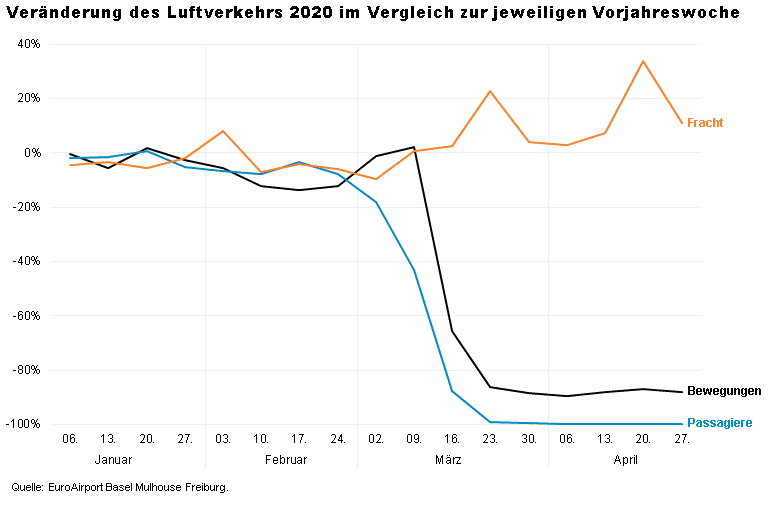
\includegraphics[height=190pt]{img_niklas/flugverkehr.PNG}
            \label{fig:my_label}
        \end{figure}
\end{frame}

\begin{frame}{CAD-Neupositionierung}
    \begin{minipage}[b]{0.7\textwidth}
    \begin{block}{Umrüstung}

    \begin{itemize}
          \item Passagierflüge durch Covid stark zurückgegangen
          \item Luftfracht ist angestiegen
          \item Boeing 777 Passagierflugzeug: 30 Tonnen Kapazität
          \item Boeing 777 Frachter: 100 Tonnen Kapazität
          \item Umrüstung von Passagierflugzeug zu Frachtmaschine
          \item Baupläne ungenau
          \item Andere Umrüstungen
      \end{itemize}
    \end{block}
    \end{minipage}
    \begin{minipage}[b]{0.27\textwidth}
        \begin{figure}
            \begin{minipage}{\textwidth}
                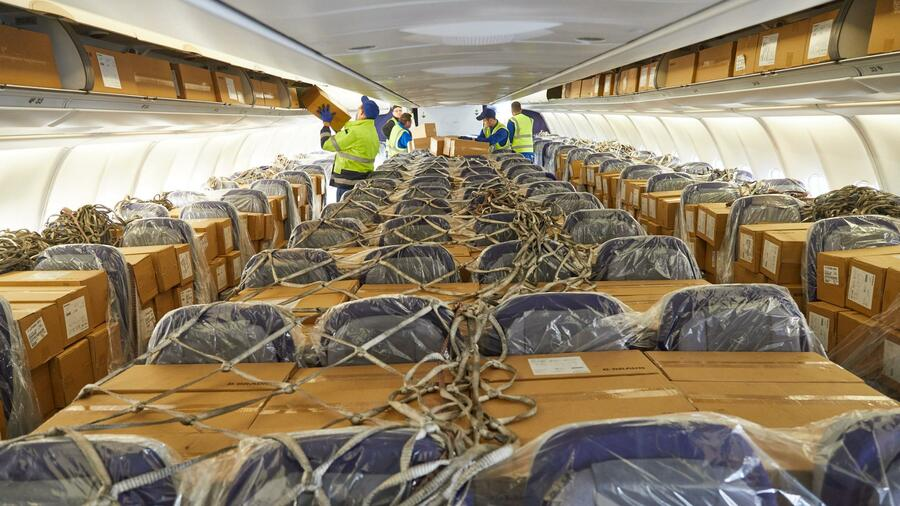
\includegraphics[width=125pt]{img_niklas/frachtMaschine.jpg}
                \label{fig:my_label}
            \end{minipage}
            \begin{minipage}{\textwidth}
                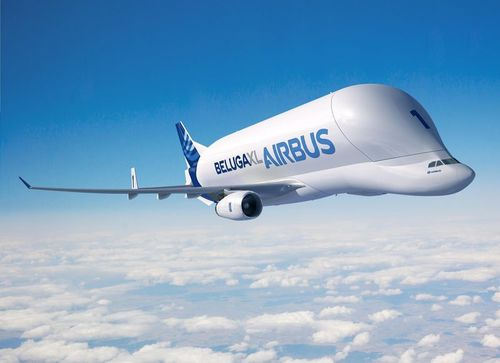
\includegraphics[width=125pt]{img_niklas/frachtFlugzeug.jpg}
            \label{fig:my_label}
            \end{minipage}
        \end{figure}
    \end{minipage}

\end{frame}

\begin{frame}{CAD-Neupositionierung}
    \begin{minipage}[]{0.5\textwidth}
    \begin{block}{Probleme}
        \begin{itemize}
            \item Baupläne oft ungenau
            \item Viele Anpassungen
            \item Großer Arbeitsaufwand
            \item Materialverschwendung
        \end{itemize}
    \end{block}
    \begin{block}{CAD-Neupositionierung}
        \begin{itemize}
            \item vorhandenes 3D Modell verbessern
            \item Genaue Planung
            \item Aufwand Minimierung
            \item Andere Nutzen
        \end{itemize}
    \end{block}
    \end{minipage}
    \begin{minipage}[]{0.49\textwidth}
      \begin{figure}
          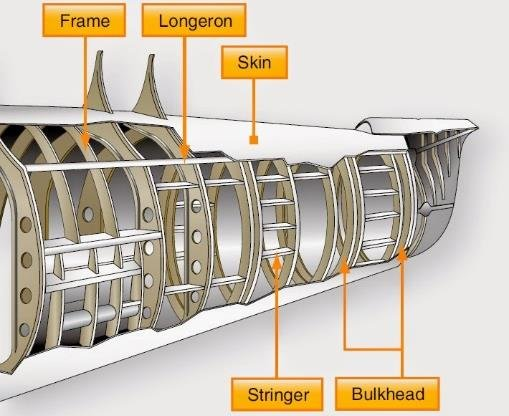
\includegraphics[width=170pt]{img_niklas/frame_Stringer.jpg}
      \end{figure}
    \end{minipage}
\end{frame}

\begin{frame}{CAD-Neupositionierung}
    \begin{minipage}[m]{0.49\textwidth}
    \begin{block}{Verfahren}
        \begin{itemize}
            \item \textbf{3D Scan und Point Cloud}
            \item Klassifizierung der Komponenten
            \item Segmentierung der Komponenten
            \item Clean up
            \item Repositionierung
            \begin{itemize}
                \item 2 Point Clouds
                \item Iterative-Closest-Point Algo.
                \item Aufsummieren des Abstands
                \item Fitness Score
            \end{itemize}
            \item Ergebnisse speichern
        \end{itemize}
    \end{block}
    \end{minipage}
    \begin{minipage}[m]{0.49\textwidth}
      \begin{figure}
          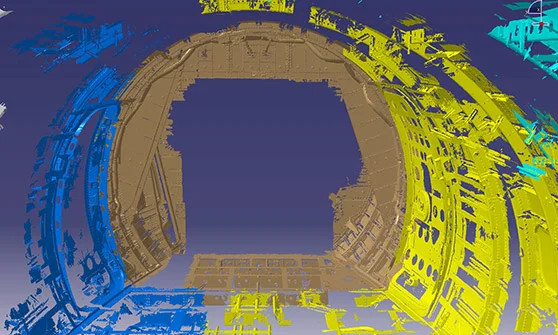
\includegraphics[width=190pt]{img_niklas/ImageForArticle_11471(1).jpg}
          \label{fig:my_label}
      \end{figure}
    \end{minipage}
\end{frame}

\begin{frame}{CAD-Neupositionierung}
    \begin{minipage}[m]{0.49\textwidth}
    \begin{block}{Verfahren}
        \begin{itemize}
            \item 3D Scan und Point Cloud
            \item \textbf{Klassifizierung der Komponenten}
            \item Segmentierung der Komponenten
            \item Clean up
            \item Repositionierung
            \begin{itemize}
                \item 2 Point Clouds
                \item Iterative-Closest-Point Algo.
                \item Aufsummieren des Abstands
                \item Fitness Score
            \end{itemize}
            \item Ergebnisse speichern
        \end{itemize}
    \end{block}
    \end{minipage}
    \begin{minipage}[m]{0.49\textwidth}
      \begin{figure}
          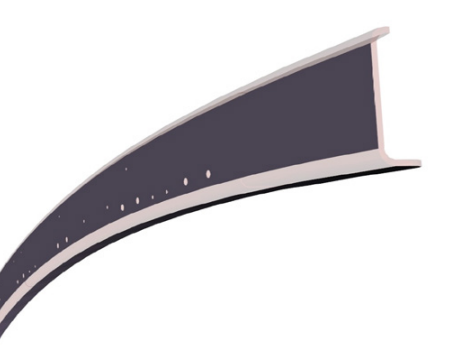
\includegraphics[width=190pt]{img_niklas/classification_frame.PNG}
          \label{fig:my_label}
      \end{figure}
    \end{minipage}
\end{frame}

\begin{frame}{CAD-Neupositionierung}
    \begin{minipage}[m]{0.49\textwidth}
    \begin{block}{Verfahren}
        \begin{itemize}
            \item 3D Scan und Point Cloud
            \item Klassifizierung der Komponenten
            \item \textbf{Segmentierung der Komponenten}
            \item Clean up
            \item Repositionierung
            \begin{itemize}
                \item 2 Point Clouds
                \item Iterative-Closest-Point Algo.
                \item Aufsummieren des Abstands
                \item Fitness Score
            \end{itemize}
            \item Ergebnisse speichern
        \end{itemize}
    \end{block}
    \end{minipage}
    \begin{minipage}[m]{0.49\textwidth}
      \begin{figure}
          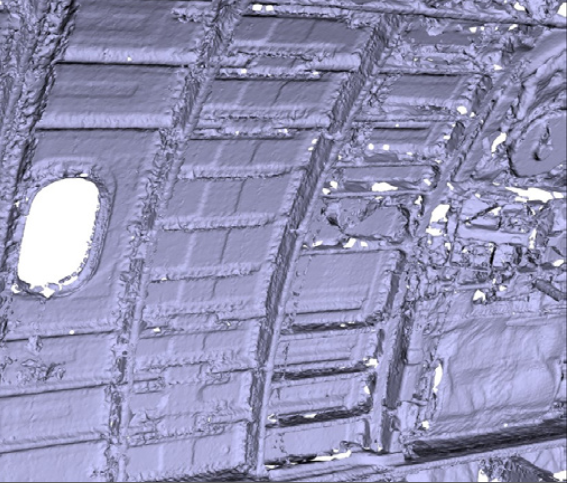
\includegraphics[width=190pt]{img_niklas/aircraft_3dscan.PNG}
          \label{fig:my_label}
      \end{figure}
    \end{minipage}
\end{frame}

\begin{frame}{CAD-Neupositionierung}
    \begin{minipage}[m]{0.49\textwidth}
    \begin{block}{Verfahren}
        \begin{itemize}
            \item 3D Scan und Point Cloud
            \item Klassifizierung der Komponenten
            \item \textbf{Segmentierung der Komponenten}
            \item Clean up
            \item Repositionierung
            \begin{itemize}
                \item 2 Point Clouds
                \item Iterative-Closest-Point Algo.
                \item Aufsummieren des Abstands
                \item Fitness Score
            \end{itemize}
            \item Ergebnisse speichern
        \end{itemize}
    \end{block}
    \end{minipage}
    \begin{minipage}[m]{0.49\textwidth}
      \begin{figure}
          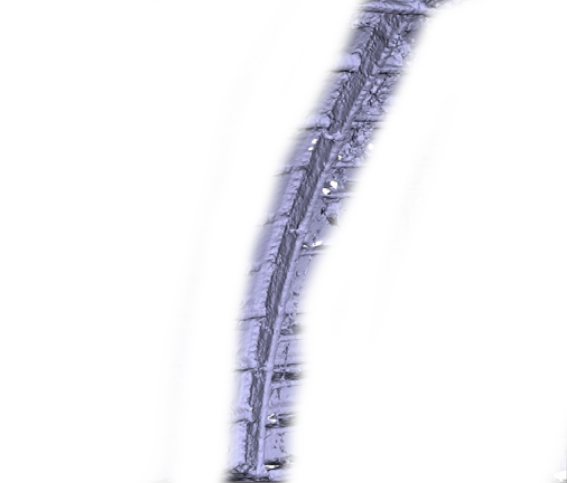
\includegraphics[width=190pt]{img_niklas/aircraft_3dscan_segmented.PNG}
          \label{fig:my_label}
      \end{figure}
    \end{minipage}
\end{frame}

\begin{frame}{CAD-Neupositionierung}
    \begin{minipage}[]{0.49\textwidth}
    \begin{block}{Verfahren}
        \begin{itemize}
            \item 3D Scan und Point Cloud
            \item Klassifizierung der Komponenten
            \item Segmentierung der Komponenten
            \item \textbf{Clean up}
            \item Repositionierung
            \begin{itemize}
                \item 2 Point Clouds
                \item Iterative-Closest-Point Algo.
                \item Aufsummieren des Abstands
                \item Fitness Score
            \end{itemize}
            \item Ergebnisse speichern
        \end{itemize}
    \end{block}
    \end{minipage}
    \begin{minipage}[]{0.49\textwidth}
      \begin{figure}
          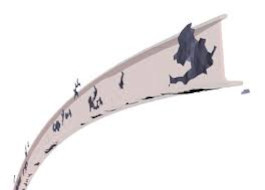
\includegraphics[width=190pt]{img_niklas/clean_up_before.jpg}
          \label{fig:my_label}
      \end{figure}
    \end{minipage}
\end{frame}

\begin{frame}{CAD-Neupositionierung}
    \begin{minipage}[]{0.49\textwidth}
    \begin{block}{Verfahren}
        \begin{itemize}
            \item 3D Scan und Point Cloud
            \item Klassifizierung der Komponenten
            \item Segmentierung der Komponenten
            \item \textbf{Clean up}
            \item Repositionierung
            \begin{itemize}
                \item 2 Point Clouds
                \item Iterative-Closest-Point Algo.
                \item Aufsummieren des Abstands
                \item Fitness Score
            \end{itemize}
            \item Ergebnisse speichern
        \end{itemize}
    \end{block}
    \end{minipage}
    \begin{minipage}[]{0.49\textwidth}
      \begin{figure}
          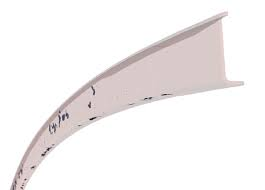
\includegraphics[width=190pt]{img_niklas/clean_up_after.jpg}
          \label{fig:my_label}
      \end{figure}
    \end{minipage}
\end{frame}


\begin{frame}{CAD-Neupositionierung}
    \begin{minipage}[]{0.49\textwidth}
    \begin{block}{Verfahren}
        \begin{itemize}
            \item 3D Scan und Point Cloud
            \item Klassifizierung der Komponenten
            \item Segmentierung der Komponenten
            \item Clean up
            \item \textbf{Repositionierung}
            \begin{itemize}
                \item 2 Point Clouds
                \item Iterative-Closest-Point Algo.
                \item Aufsummieren des Abstands
                \item Fitness Score
            \end{itemize}
            \item Ergebnisse speichern
        \end{itemize}
    \end{block}
    \end{minipage}
    \begin{minipage}[]{0.49\textwidth}
      \begin{figure}
          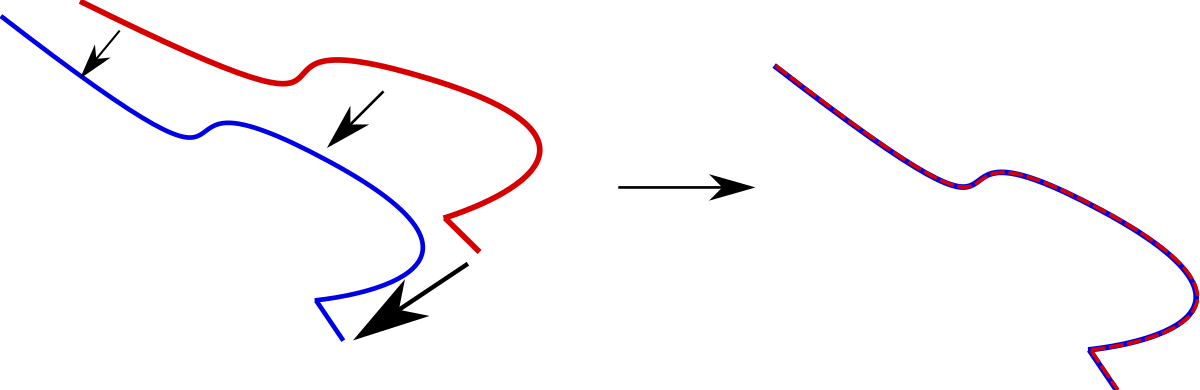
\includegraphics[width=190pt]{img_niklas/1200px-Idea_closest_point_algorithm.svg.png}
          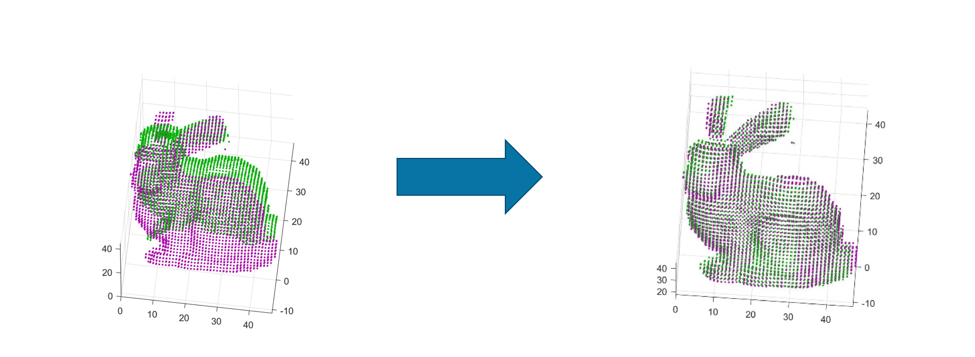
\includegraphics[width=190pt]{img_niklas/icp_3d.png}
          \label{fig:my_label}
      \end{figure}
    \end{minipage}
\end{frame}

\begin{frame}{CAD-Neupositionierung}
    \begin{minipage}[]{0.49\textwidth}
    \begin{block}{Verfahren}
        \begin{itemize}
            \item 3D Scan und Point Cloud
            \item Klassifizierung der Komponenten
            \item Segmentierung der Komponenten
            \item Clean up
            \item Repositionierung
            \begin{itemize}
                \item 2 Point Clouds
                \item Iterative-Closest-Point Algo.
                \item Aufsummieren des Abstands
                \item Fitness Score
            \end{itemize}
            \item \textbf{Ergebnisse speichern}
        \end{itemize}
    \end{block}
    \end{minipage}
    \begin{minipage}[]{0.49\textwidth}
      \begin{figure}
          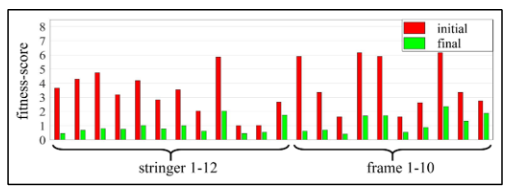
\includegraphics[width=190pt]{img_niklas/results_repo.PNG}
          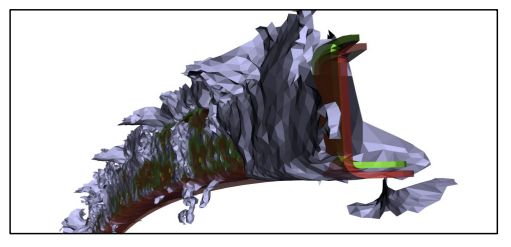
\includegraphics[width=190pt]{img_niklas/inital_vs_final.PNG}
          \label{fig:my_label}
      \end{figure}
    \end{minipage}
\end{frame}

\begin{frame}{CAD-Neupositionierung}
    \begin{block}{Zusammenfassung}
        \begin{itemize}
            \item Kombination von schon vorhandenem
            \item Open-Source
            \item Automatisierung
            \item Verbessert Modelle
            \item Minimiert Arbeitsaufwand
            \item Indikator für Modelle
        \end{itemize}
    \end{block}
\end{frame}

\begin{frame}{CAD-Neupositionierung}
\begin{figure}
    \centering
    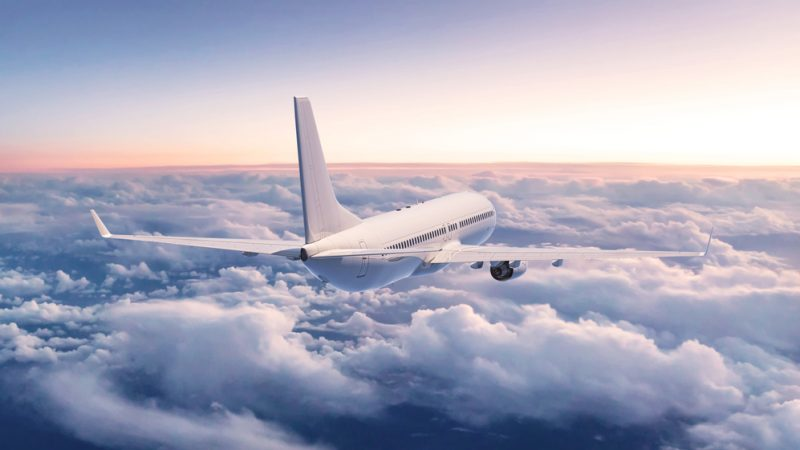
\includegraphics[height=175pt]{img_niklas/end_frame.jpg}
    \caption*{Danke fürs Zuhören}
    \label{fig:my_label}
\end{figure}

\end{frame}